% https://tex.stackexchange.com/questions/246/when-should-i-use-input-vs-include
% \input is a more lower level macro which simply inputs the content of the given file like it was copy&pasted there manually. \include handles the file content as a logical unit of its own (like e.g. a chapter) and enables you to only include specific files using \includeonly{filename,filename2,...} to save times.

% Long answer:
% The \input{<filename>} macro makes LaTeX to process the content of the given file basically the same way as if it would be written at the same place as \input. The LaTeX version of \input only does some sanity checks and then uses the TeX \input primitive which got renamed to \@@input by LaTeX.

% Mentionable properties of \input are:

% You can use \input basically everywhere with any content.
% It is usable in the preamble, inside packages and in the document.
% You can nest \input macros.
% You can use \input inside a file which is read using \input.
% The only thing \input does is to input the file.
% You don't have to worry about any side effects, but don't get any extra features.
% The \include{<filename>} macro is bigger and is supposed to be used with bigger amounts of content, like chapters, which people might like to compile on their own during the editing process.

% \include does basically the following thing:

% It uses \clearpage before and after the content of the file. This ensure that its content starts on a new page of its own and is not placed together with earlier or later text.
% It opens a new .aux file for the given file.
% There will be a filename.aux file which contains all counter values, like page and chapter numbers etc., at the begin of the filename. This way the file can be compiled alone but still has the correct page and chapter etc. numbers. Such part aux files are read by the main aux file.
% It then uses \input internally to read the file's content.
% Mentionable properties of \include are:

% It can't be used anywhere except in the document and only where a page break is allowed.
% Because of the \clearpage and the own .aux file \include doesn't work in the preamble, inside packages. Using it in restricted modes or math mode won't work properly, while \input is fine there.
% You can't nest \include files.
% You can't use \include inside a file which is read by \include. This is by intention and is because to avoid issues with the .aux files. Otherwise three .aux files (main, parent \include, child \include) would be open at the same time which was deemed to complicated I guess.
% You can use \input inside an \include file and also \input an \include file.
% Biggest benefit: You can use \includeonly{filename1,filename2,...} in the preamble to only include specific \include files.
% Because the state of the document (i.e. above mentioned counter values) was stored in an own .aux file all page and sectioning numbers will still be correct. This is very useful in the writing process of a large document because it allows you to only compile the chapter you currently write on while skipping the others. Also, if used persistently it can be used to create PDFs of sub-parts of your document, like only the front matter or everything but/only the appendix, etc.
% There is also the excludeonly package which provides an \excludeonly to exclude only certain files instead of including all other files.
\documentclass[12pt]{book}
\usepackage{import} % import – Establish input relative to a directory
\usepackage{graphicx}
\usepackage{listings}
\usepackage{emptypage}
\usepackage{blindtext}


% \includeonly{24-multi-files-chapter-one, 24-multi-files-chapter-three}


\begin{document}


\tableofcontents
\listoffigures


% METHOD ONE
\chapter{Introduction}

\section{Who am I}
\blindtext

\section{What I do}
\Blindtext[2]

\chapter{The Solution}



\section{Brief}

\blindtext

\begin{table}[ht]
    \centering
        \begin{tabular}{c | c | c}
            Name & Strengths & Weaknesses \\
            \hline
            Old but Gold & Popular & Lack of features \\
            New and Fresh & Whole new architecture & Lack of community supports
        \end{tabular}
    \caption{Strengths and Weaknesses of Methods}
    \label{tab:method summary}
\end{table}

\blindtext

\begin{figure}[ht]
    \centering
    
\includegraphics[width=8cm]{img/nextvoyage-road-moutain.jpg}
    \caption{Road Heading Towards Mountain by Nextvoyage}
    \label{fig:purple flower}
\end{figure}

\blindtext



\section{Conclusion}

\Blindtext[2]

\chapter{Topics for further reading}



\section{Our context}

\blindtext

\begin{lstlisting}[language=Python, caption={Nested for loop in Python}, captionpos=b]
for i in range(5):
    for j in range(2):
        # Print a string
        print(f'i={i}, j={j}')
\end{lstlisting}

\blindtext



\section{The topics}



\subsection{Topic A}

\blindtext

\begin{figure}[ht]
    \centering
    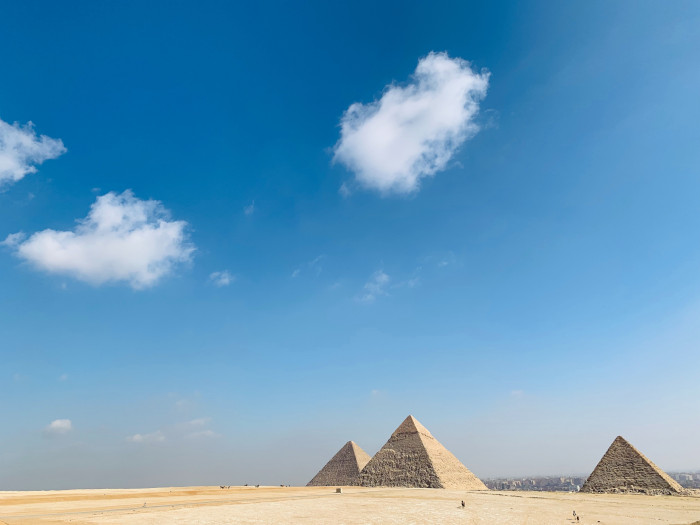
\includegraphics[width=8cm]{img/dave-ang-pyramid.jpg}
    \caption{Three Great Pyramid Under The Blue Sky by Dave Ang}
    \label{fig:great_pyramid}
\end{figure}

\blindtext



\subsection{Topic B}

\Blindtext[2]

\begin{figure}[ht]
    \centering
    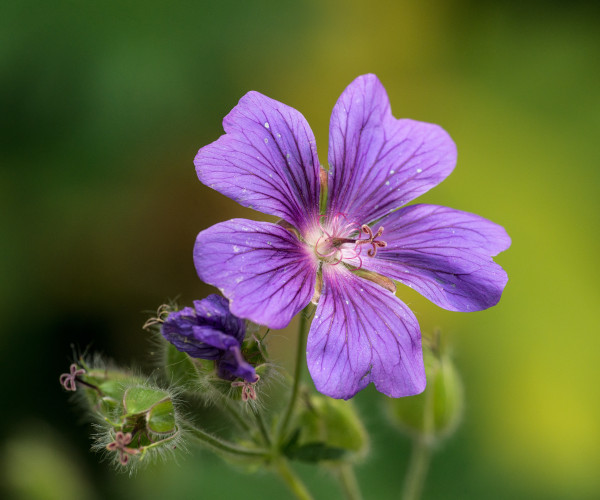
\includegraphics[width=\textwidth]{img/ganajp-purple-flower.jpg}
    \caption{Purple Flower by Petr Ganaj}
    \label{fig:purple_flower}
\end{figure}

\blindtext


% METHOD TWO
% \chapter{Introduction}

\section{Who am I}
\blindtext

\section{What I do}
\Blindtext[2]

% \chapter{The Solution}



\section{Brief}

\blindtext

\begin{table}[ht]
    \centering
        \begin{tabular}{c | c | c}
            Name & Strengths & Weaknesses \\
            \hline
            Old but Gold & Popular & Lack of features \\
            New and Fresh & Whole new architecture & Lack of community supports
        \end{tabular}
    \caption{Strengths and Weaknesses of Methods}
    \label{tab:method summary}
\end{table}

\blindtext

\begin{figure}[ht]
    \centering
    
\includegraphics[width=8cm]{img/nextvoyage-road-moutain.jpg}
    \caption{Road Heading Towards Mountain by Nextvoyage}
    \label{fig:purple flower}
\end{figure}

\blindtext



\section{Conclusion}

\Blindtext[2]

% \chapter{Topics for further reading}



\section{Our context}

\blindtext

\begin{lstlisting}[language=Python, caption={Nested for loop in Python}, captionpos=b]
for i in range(5):
    for j in range(2):
        # Print a string
        print(f'i={i}, j={j}')
\end{lstlisting}

\blindtext



\section{The topics}



\subsection{Topic A}

\blindtext

\begin{figure}[ht]
    \centering
    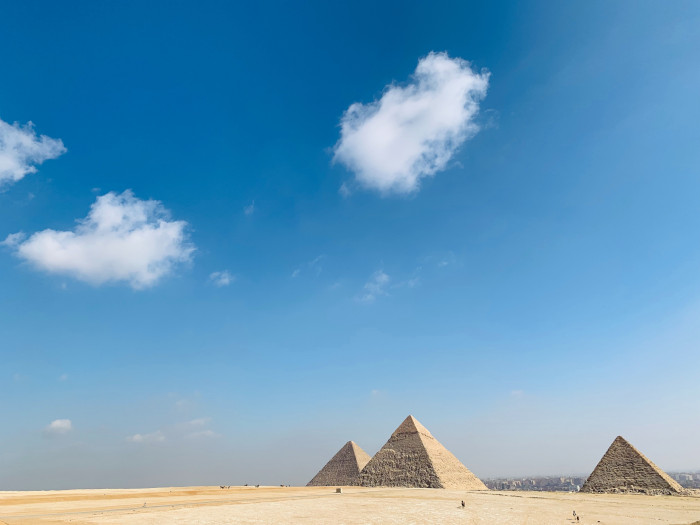
\includegraphics[width=8cm]{img/dave-ang-pyramid.jpg}
    \caption{Three Great Pyramid Under The Blue Sky by Dave Ang}
    \label{fig:great_pyramid}
\end{figure}

\blindtext



\subsection{Topic B}

\Blindtext[2]

\begin{figure}[ht]
    \centering
    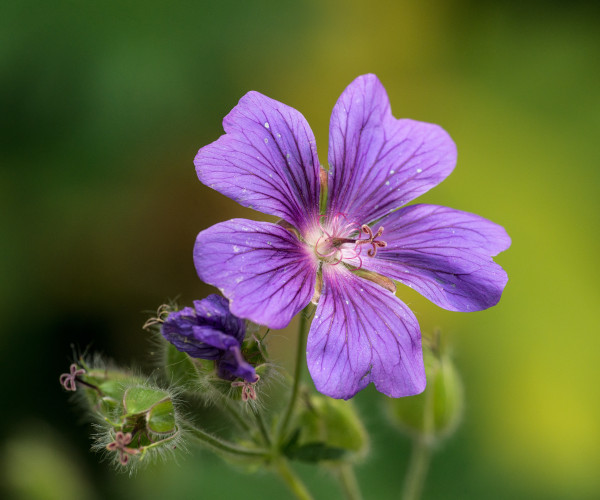
\includegraphics[width=\textwidth]{img/ganajp-purple-flower.jpg}
    \caption{Purple Flower by Petr Ganaj}
    \label{fig:purple_flower}
\end{figure}

\blindtext


% METHOD THREE
% \import{./}{24-multi-files-chapter-one}
% \import{./}{24-multi-files-chapter-two}
% \import{./}{24-multi-files-chapter-three}


\end{document}
